%%%%%%%%%%%%%%%%%%%%%%%%%%%%%%%%
%%%
%%% Research Summary
%%%
%%% Author - Steve Hurder
%%%
%%% Date Started: October 12, 2009
%%% Date Completed: November 15 , 2009
%%%%%%%%%%%%%%%%%%%%%%%%%%%%%%%%

\documentclass[11pt]{amsart}
\usepackage{graphicx}
\usepackage{amssymb}
\usepackage{colortbl}
\usepackage{epstopdf}
\usepackage{url}


\usepackage[top=1in, bottom=1in, left=1in, right=1in]{geometry}

\newcommand{\student}[1]{\vspace{.5cm}\fbox{\parbox{0.95\linewidth}{{\small
        #1}}}\vspace{.5cm}}
\providecommand{\blue}[1]{{\color{blue}{#1}}}
\providecommand{\red}[1]{{\color{red}{#1}}}
\providecommand{\green}[1]{{\color{green}{#1}}}

\begin{document}

 \title{How Natural Language Processing can Open Machine Learning's Black Box}

 \author{Jordan Boyd-Graber, University of Maryland}
%\institute{University of Colorado, Boulder CO 80309, USA}


\date{Fall 2020}

\maketitle

Machine learning is ubiquitous: detecting spam e-mails, flagging fraudulent
purchases, and providing the next movie in a Netflix binge.  But few at
the mercy of machine learning \emph{outputs} know what's happening behind the
curtain.  My research goal is to demystify the black box for non-experts by
creating \emph{algorithms that can inform, collaborate with, compete with, and
  understand users} in real-world settings.

This is at odds with mainstream machine learning---take topic models.  Topic
models are sold as a tool for understanding large data collections: lawyers
scouring Nordstream e-mails for a smoking gun, journalists making sense of Wikileaks,
or humanists characterizing the oeuvre of Lope de Vega.  But topic models'
proponents never asked what those lawyers, journalists, or humanists
needed. Instead, they optimized \emph{held-out likelihood}. When my colleagues
and I developed the \emph{interpretability} measure to assess whether topic
models' users understood their outputs, interpretability and
held-out likelihood were negatively correlated~\cite{chang-09b}! The topic
modeling community (including me) had fetishized complexity at the expense of
usability\dots and topic modeling is not alone, question answering has distinct but similar issues with evaluation~\cite{boyd-graber-20}.

\begin{center}
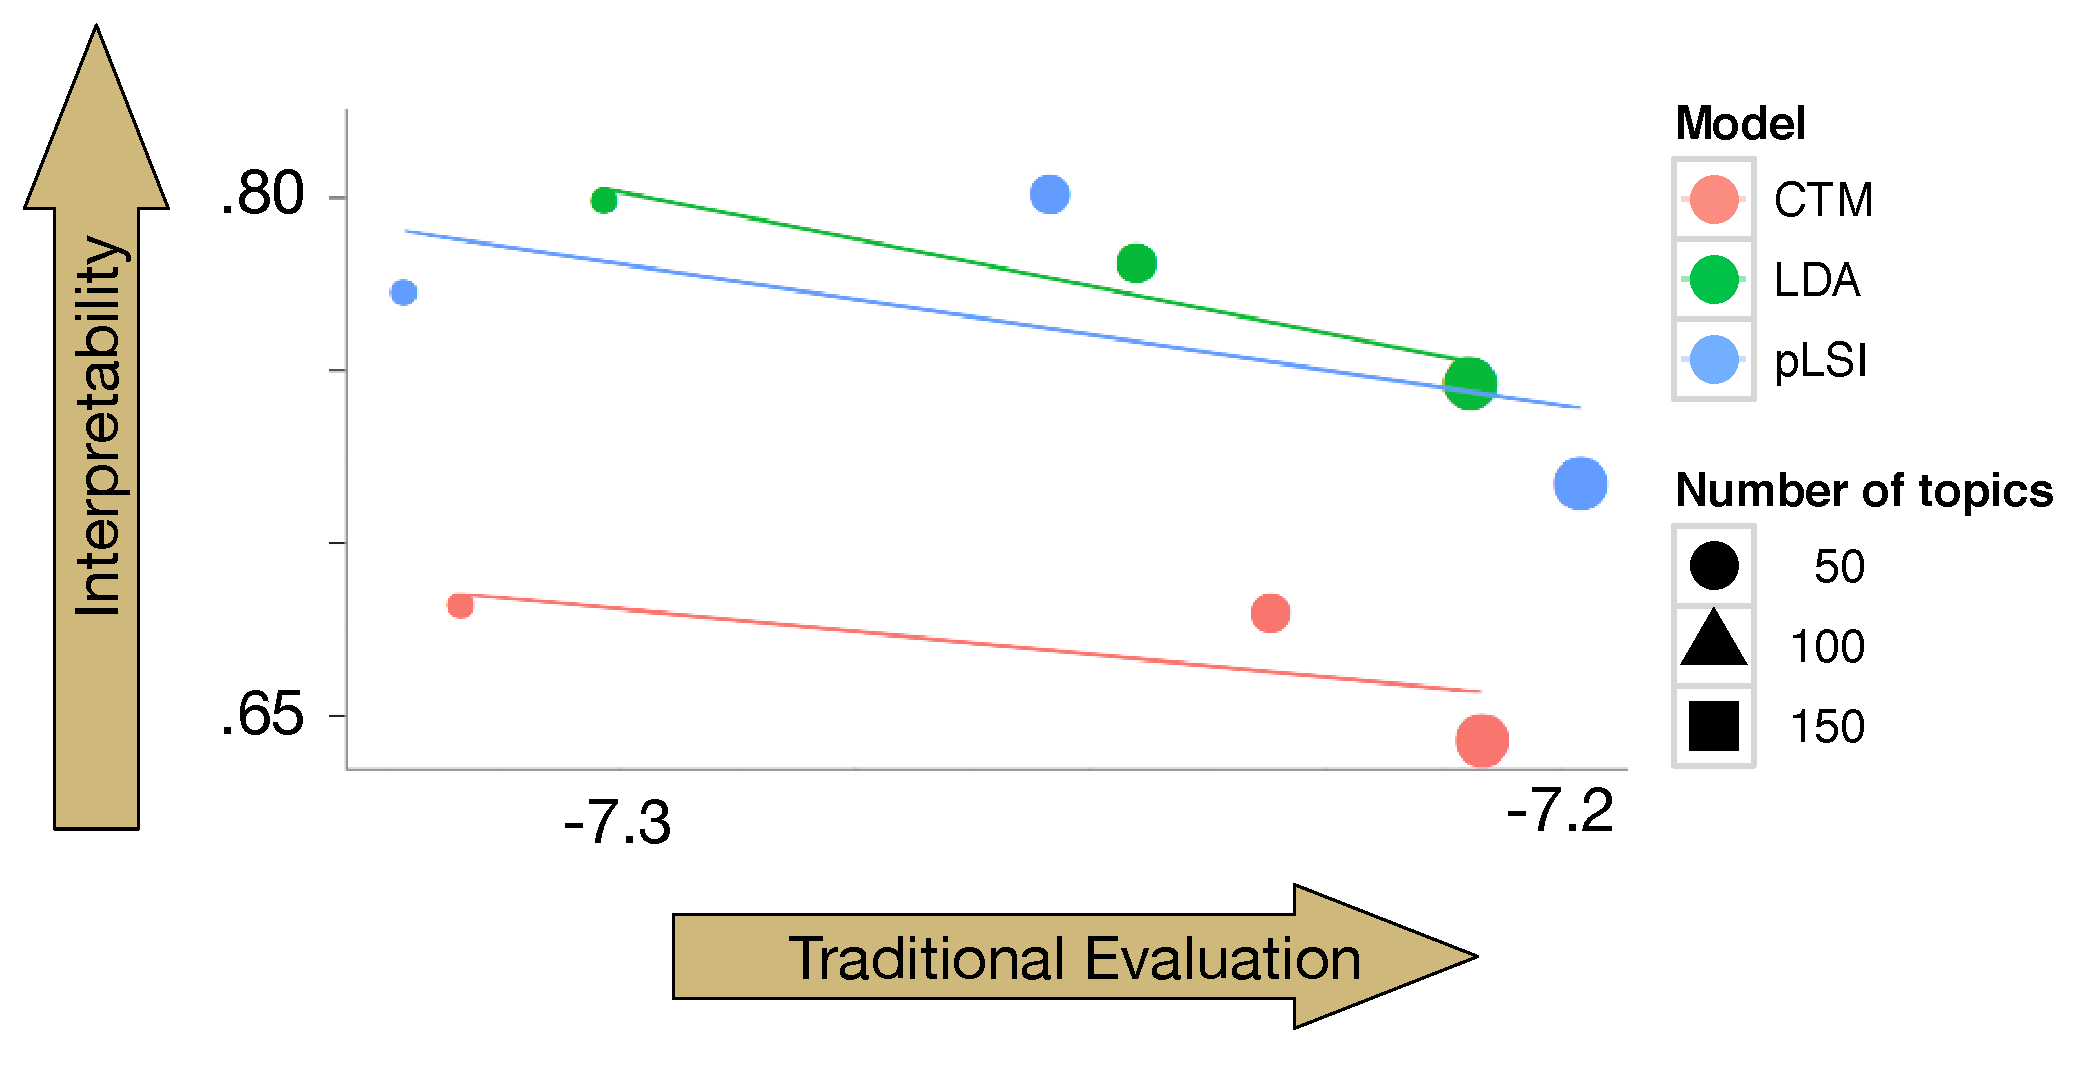
\includegraphics[width=.5\linewidth]{images/prec_ll_4}
\end{center}

Since this humbling discovery, I've built topic models that are a collaboration
between humans and computers.  The computer starts by proposing an organization
of the data.  The user separates confusing clusters or joins
similar clusters together~\cite{hu-14:itm}.  The model updates and directs the user to
problematic areas that.  This is a huge improvement over the
``take it or leave it'' philosophy of most machine learning algorithms.

This is not only a technical improvement but also an improvement to the social
process of machine learning adoption. Our tools allow non-experts to fix such obvious (to
a human) problems, allowing machine learning algorithms to overcome the
\emph{social} barriers that often hamper adoption.

\begin{minipage}[b]{0.4\textwidth}
\begin{tabular}{p{.9\textwidth}}
	Topic Words (before) \\
\hline
 \red{bladder}, sci, \blue{spinal\_cord}, \blue{spinal\_cord\_injury}, \blue{spinal}, \red{urinary}, \red{urinary\_tract}, \red{urothelial},\blue{injury}, \blue{motor}, \blue{recovery}, \blue{reflex}, \blue{cervical}, \red{urothelium}, \blue{functional\_recovery} \\
\end{tabular}
\end{minipage}
  \hfill
\begin{minipage}[b]{0.4\textwidth}
\begin{tabular}{p{.9\textwidth}}
	Topic Words (after) \\
\hline
sci, \blue{spinal\_cord}, \blue{spinal\_cord\_injury}, \blue{spinal}, \blue{injury}, \blue{recovery}, \blue{motor}, \blue{reflex}, \red{urothelial}, \green{injured}, \blue{functional\_recovery}, \green{plasticity}, \green{locomotor}, \blue{cervical}, \green{locomotion}\\
\end{tabular}
\end{minipage}

% Fix ``on the fly''

Another shortcoming of interactive machine learning models is that they are
often too slow. We developed methods that go beyond traditional proababilistic
interpretations. We extend the geometric interpretations of admixture models
developed by Arora et al.~\cite{arora-12} to multi-anchor topics~\cite{lund-17}
and multi-lingual topics~\cite{Yuan-18}. We have also developed better
understanding of projection-based multilingual representations via graph
theory~\cite{Fujinuma-19} and the convergence of alternating
projections~\cite{Zhang-19}.

However, lexicons are not the only way humans can teach machines: reinforcement learning can capture humans' subtle strategies.
\emph{Simultaneous machine
  interpretation}~\cite{Grissom:He:Boyd-Graber:Morgan-2014} is another
language-based task that requires significant human intuition,
insight, and---for those who want to become
interpreters---training. Because verbs end phrases in many languages,
such as German and Japanese, existing algorithms must wait until the
end of a sentence to begin translating (since English sentences have
verbs near the start). We learned tricks from professional human
interpreters---passivizing sentences and guessing the verb---to
translate sentences sooner~\cite{He-15}, letting speakers and
algorithms cooperate together and enabling more natural cross-cultural
communication.  We can also use reinforcement learning to learn
machine translation feedback from noisy supervision such as star
ratings on a webpage~\cite{nguyen-17}.

The reverse of cooperation is competition; it also has much to teach computers.
I've increasingly looked at language-based games whose clear goals and
intrinsic fun speed research progress. For example, in \emph{Diplomacy}, users
chat with each other while marshaling armies for world conquest. Alliances are
fluid: friends are betrayed and enemies embraced as the game develops. However,
users' conversations let us predict when friendships break: betrayers writing
ostensibly friendly messages before a betrayal become more polite, stop talking
about the future, and change how much they write~\cite{niculae-15} in follow-on
work, we develop a dataset that helps predict both when users lie to each other
and when recipients of lies detect deception~\cite{Peskov-20}. Diplomacy may be
a nerdy game, but it is a fruitful testbed to teach computers to understand
messy, emotional human interactions.

A game with higher stakes is politics. However, just like Diplomacy, the words
that people use reveal their underlying goals; computational methods can help
expose the ``moves'' political players can use. With collaborators in political
science, we've built models that: show when politicians in debates
strategically change the topic to influence others~\cite{nguyen-12,Nguyen-14b};
frame topics to reflect political leanings~\cite{nguyen-13:shlda}; use subtle
linguistic phrasing to express their political leaning~\cite{iyyer-14a}; or
create political subgroups with larger political
movements~\cite{Nguyen:Boyd-Graber:Resnik:Miler-2015}.

Conversely, games also teach humans \emph{how computers think}.  Our
trivia-playing robot~\cite{boyd-graber-12,iyyer-14b,iyyer-15} faced off against
former Jeopardy champions in front of hundreds high school
students.\footnote{\url{https://www.youtube.com/watch?v=LqsUaprYMOw}} The
computer claimed an early lead, but we foolishly projected the computer's
thought process for all to see.  The humans learned to read the algorithm's
ranked dot products and schemed to answer just before the computer. In five
years of teaching machine learning, I've never had students catch on so quickly
to how linear classifiers work.  The probing questions from high school students
in the audience showed they caught on too.  Later, when we played again against
Ken Jennings,\footnote{\url{https://www.youtube.com/watch?v=kTXJCEvCDYk}} he sat
in front of the dot products and our system did much better.  However,
much of computers' advantage comes from repeated word overlaps in
questions~\cite{wallace-19}.

I recently outlined how we can improve measurement of question
answering progress~\cite{boyd-graber-20}.  With Pedro Rodriguez, we
are combining the question-level adversarial techniques with insights
from item-response theory to capture: what questions humans find
difficult, what questions computers find difficult, and what
\emph{test} sets can most efficiently identify how well an agent can
answer questions.  This can help spur more focused machine learning
research to focus on important problems (for example, existing test
sets for question answering are overwhelmingly male and American\dots
accuracy for other groups is lower) and for humans, quickly identify
which topics someone knows (or not), which can aid educational
applications.

  \begin{minipage}[b]{0.4\textwidth}
    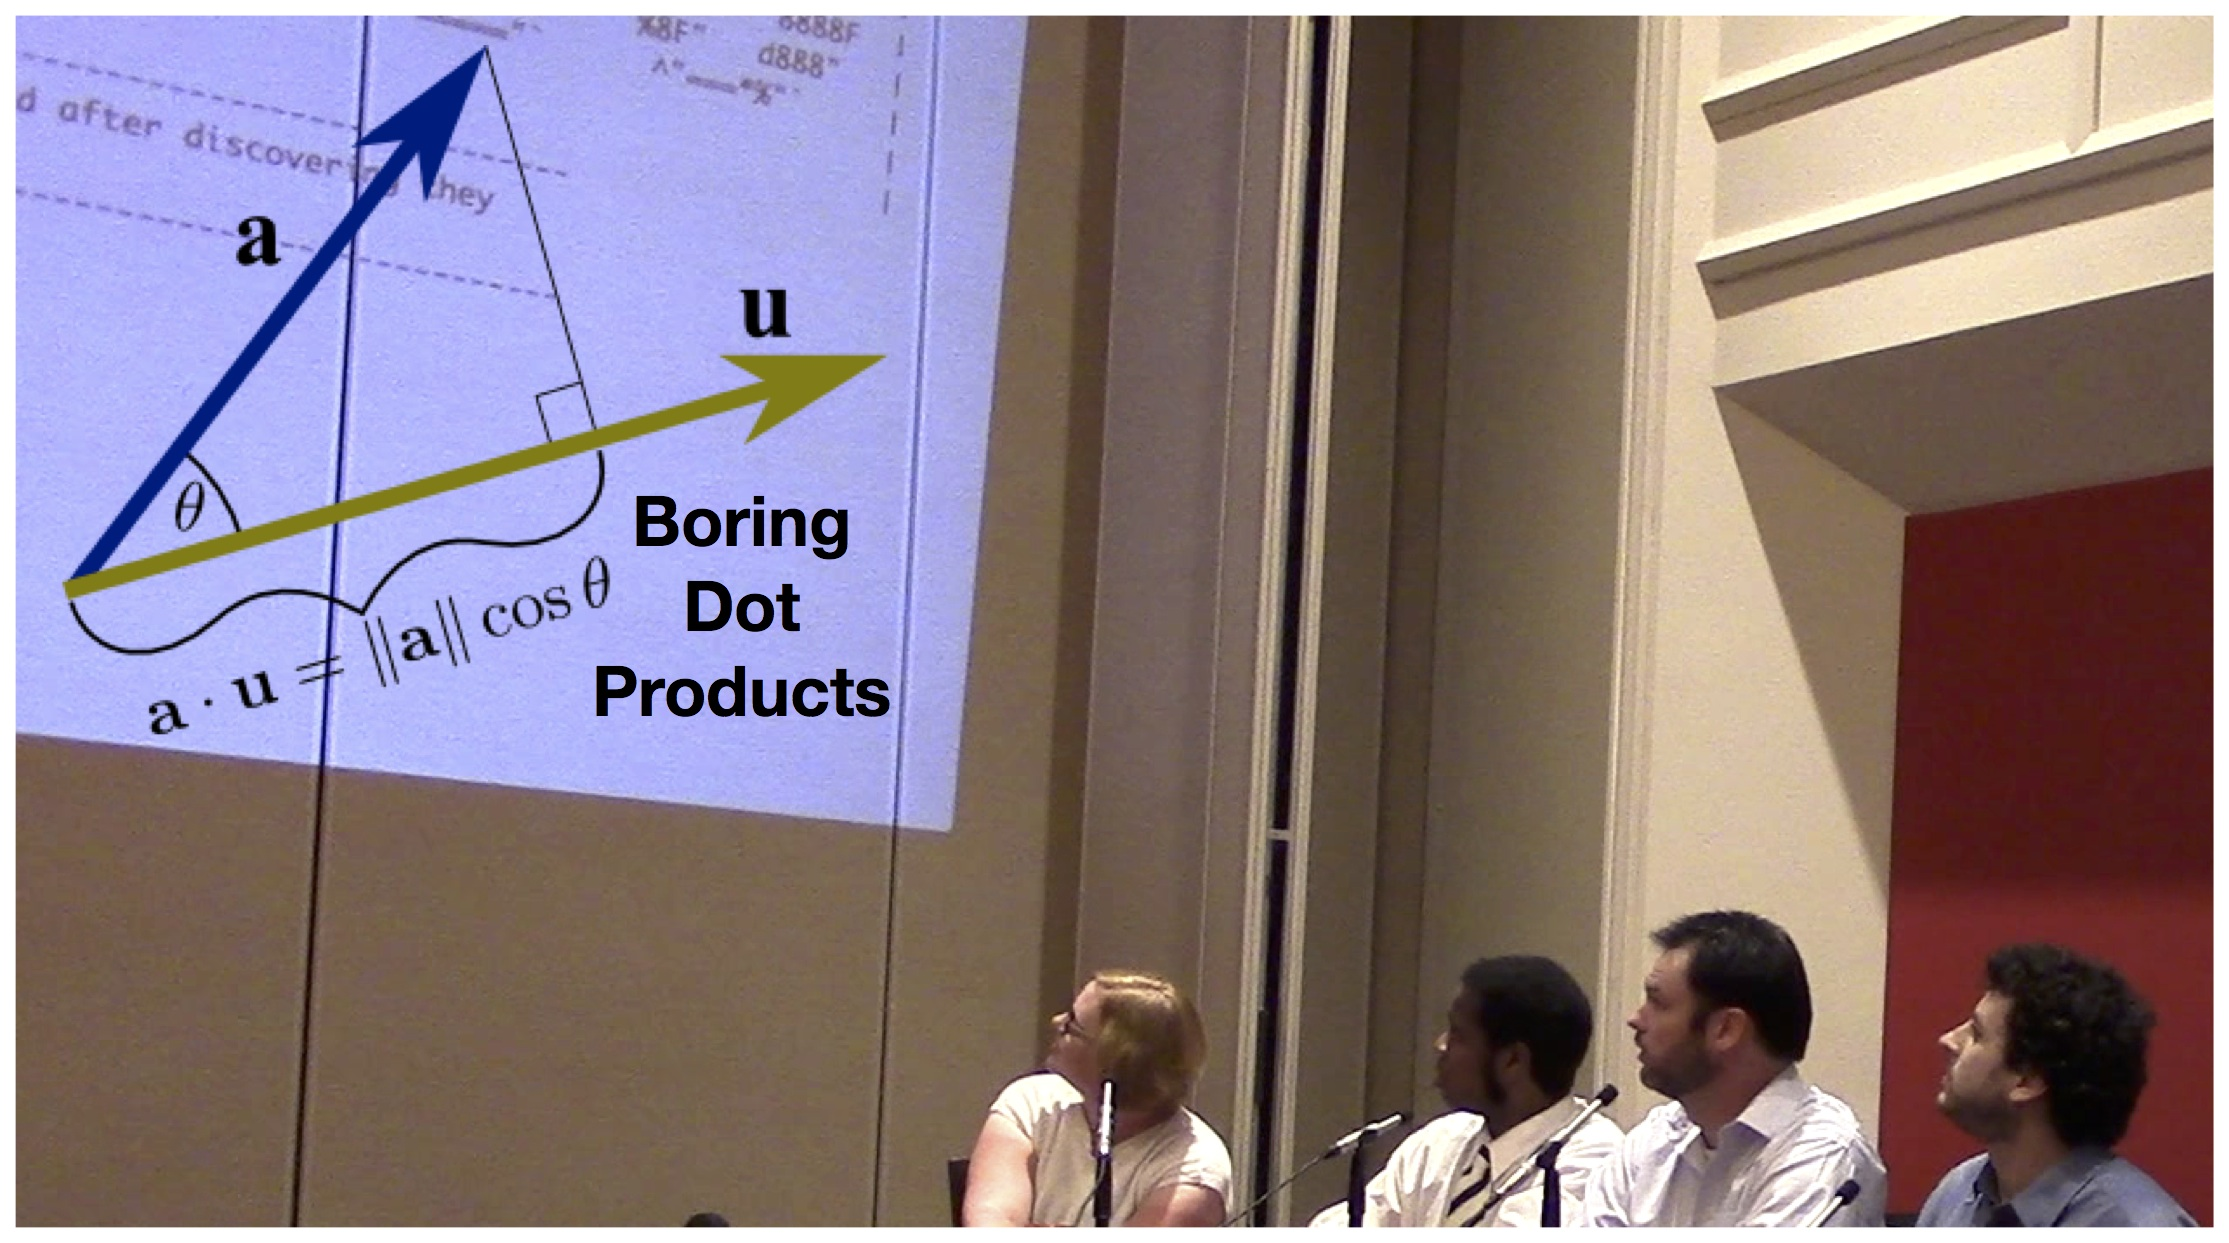
\includegraphics[width=\textwidth]{images/boring_dot_products}
  \end{minipage}
  \hfill
\begin{minipage}[b]{0.4\textwidth}
    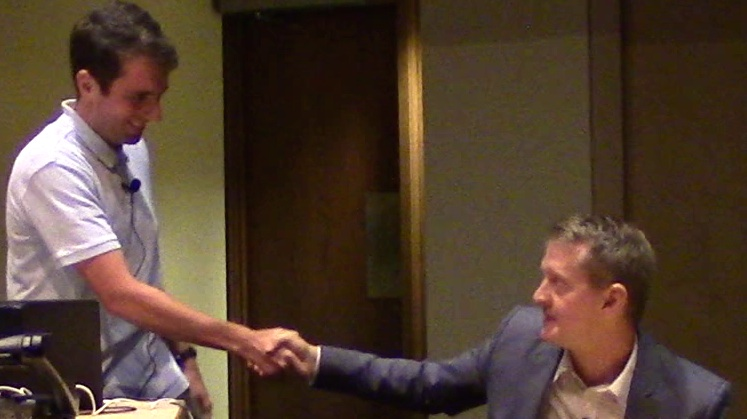
\includegraphics[width=\textwidth]{images/jennings_handshake}
  \end{minipage}

Advancing machine learning requires closer, \emph{more natural interactions}.
However, we still require much of the user---reading distributions or dot
products---rather than natural interactions. Document exploration tools should
describe in words what a cluster is, not just provide inscrutable word clouds.
Deception detection systems should say \emph{why} a betrayal is imminent.
Question answers should explain \emph{how} it knows Aaron Burr shot Alexander
Hamilton: thus helping human players of trivia games either as a study partner
or as a teammate at a competition. Likewise, users should be able to
communicate correct when algorithms go wrong naturally.

User interactions are still important---machine learning is not yet able to
extract all it needs from large datsets. But the size of this data requires us
to use the limited time and patience of user annotation. With my
student Michelle Yuan, I am developing
variants of active learning that---rather than look at whether an example
confuses a downstream classifier---look for examples that surprise language
models trained on webscale data~\cite{devlin-19}. We can then ask users to
provide feedback on the data or clusters~\cite{poursabzi-16} that language
models cannot handle.

Creating metrics to measure interpretability and systems that implement it is
the subject of my \textsc{nsf career} grant. By creating teams of humans and
computers working together to solve language problems
incrementally~\cite{feng-19}, we will extend these metrics to other
applications areas to measure how much machine learning systems (and their
visualizations) help or hurt the accuracy of their human teammates. Given a set
of pre-defined visualizations, we can use bandit algorithms to select which
visualizations are best in a particular context: an expert is more likely to
use nearest-neighbor examples, a novice is more likely to be helped by an
$n$-best list, etc. As we move beyond a set of pre-defined visualizations,
interpretability metrics can then become the reward function for reinforcement
learning to optimize the details of machine learning explanations. This
complements machine learning's ubiquity with transparent, empathetic, and
useful interactions with users.



%% \vspace{12cm}

%%  \parbox{\linewidth}{I certify that this
%%   statement is a current and accurate statement of my
%%   professional record to the best of my
%%   knowledge \flushright  
\includegraphics[width=.2\linewidth]{resume_src/signature} \\
%% \flushright  (\today{})}

\clearpage

%%%%%%%%%%%%%%%%%%%%%%%%%%%%%%%%

\bibliographystyle{resume_src/splncs03}

\begin{center}
Full list of  three book chapters, eleven journal publications, and eighty-five conference
publications at \url{http://boydgraber.org/dyn-pubs/year.html}
\end{center}

%\bibliographystyle{unsrtnat}
\bibliography{resume_src/journal-full,resume_src/jbg}
\noindent\rule{4cm}{0.4pt}
\end{document}
